\documentclass[12pt, twoside]{report}
\usepackage[a4paper, top=3cm, bottom=3cm]{geometry}
\usepackage[utf8]{inputenc}
\usepackage[T1,T2A,TS1]{fontenc}
\usepackage[russian]{babel}
\usepackage{setspace}
\usepackage{fancyhdr}
\usepackage{tocloft}
\usepackage{color}
\usepackage{footnote}
\usepackage{url}
\usepackage{babelbib}
\usepackage{array,longtable}
\usepackage{fontenc}
\usepackage{mathtext}
\usepackage{amsmath}
\usepackage{amssymb}
\usepackage{mathtools}
\usepackage[pdftex]{graphicx}
\usepackage{textcomp}
\usepackage{indentfirst}
\usepackage{cite}
\usepackage{longtable}
\usepackage{listings}
\usepackage{lipsum}
\usepackage[none]{hyphenat}
\usepackage[hypcap]{caption}
\usepackage{pdflscape}
\usepackage[citecolor = blue]{hyperref}
\usepackage{alltt}
\usepackage{ifxetex}
\usepackage[final]{pdfpages}
\usepackage{wrapfig}
%%\usepackage{svg}
%------------------Font specification-------------------%
% If you want to use font other than the default one,
% you MUST use XeLaTeX to compile.
\ifxetex
\usepackage{fontspec}
\usepackage{xunicode}
% Use Monaco as default font, change down below (if you wish).
\newfontfamily{\monaco}{Monaco} % Replace "Monaco" with another font name.
\else
\newcommand{\monaco}{\ttfamily }
\fi

\renewcommand{\lstlistingname}{Код}
\newcommand{\mysinglespacing}{%
\setstretch{1}% no correction afterwards
}


%\setlength{\hoffset}{1.5 cm}
%\setlength{\voffset}{-2 em}
%\setlength{\topmargin}{0 cm}
%\setlength{\headheight}{1 em}
%\setlength{\headsep}{1 em}
%\setlength{\oddsidemargin}{0 cm}
%\setlength{\textwidth}{16 cm}
%\setlength{\textheight}{24.7 cm}


\lstloadlanguages{C++}
\definecolor{nsclass}{RGB}{124,32,176}
\definecolor{atnotation}{RGB}{27, 103, 224}
\definecolor{import}{RGB}{128,70,30}
\definecolor{comment}{RGB}{0,140,0}
\definecolor{string}{RGB}{229,0,0}
\definecolor{method}{RGB}{70,0,134}
\definecolor{class}{RGB}{59,131,138}
\definecolor{custommethod}{RGB}{32,90,95}
\definecolor{number}{RGB}{56,0,225}
\definecolor{customgray}{RGB}{211,211,211}
\definecolor{namespaces}{RGB}{2, 153, 19}
\definecolor{number}{RGB}{227, 146, 7}
\lstset{
language=C++, tabsize=2, keepspaces=false,
xleftmargin=0em,xrightmargin=-1em, aboveskip=1em, % Margin adjustment
%backgroundcolor=\color{customgray},    % Background color (Default:gray)
%backgroundcolor=none,
 frame=none,                            % Frame not needed
breakindent=22pt,
 inputencoding=utf8,
 extendedchars=true,
%numbers=left,stepnumber=1,numberstyle=\tiny\color{black}\monaco,
basicstyle=\mysinglespacing\fontsize{11.5pt}{1em}\selectfont\monaco,
commentstyle=\fontsize{11.5pt}{0.75em}\selectfont\monaco\color{comment},
showspaces=false,
flexiblecolumns=true,
breaklines=true,
 %breakautoindent=true, breakindent=4em,
escapeinside={/*@}{@*/},
morecomment=[s][\color{string}]{"}{"},
 morecomment=[s][\color{string}]{'}{'},
morecomment=[l][\color{import}]{\#},
morecomment=**[s][\color{nsclass}]{NS}{];},
morecomment=**[s][\color{nsclass}]{UI}{];},
morecomment=**[s][\color{nsclass}]{NS}{(},
morecomment=**[s][\color{nsclass}]{UI}{)},
morecomment=**[s][\color{nsclass}]{UI}{*},
morecomment=**[s][\color{nsclass}]{NS}{*},
morecomment=*[s][\color{nsclass}]{UI}{\ },
morecomment=*[s][\color{nsclass}]{NS}{\ },
}
% Down below, you can add your custom class names / method names as presented
% in your source code.
% For example, you have two custom class names called User and Person.
% You should add in the list User, Person
% The list of names should be seperated by commas, and no quotation
% marks are required.
\lstset{
emph=[1]{  % <--Add your own Class Names before the percentage mark
cout, cin, cerr, endl
},
emphstyle=[1]{\color{class}},
emph=[2]{ % <--Add your namespaces
std
},
emphstyle=[2]{\color{namespaces}},
moreemph=[5]{ % <--Add your own Method Names before the percentage mark
},
emphstyle=[5]{\color{method}},
}

\lstset{
emph=[3]{
 @implementation,@synthesize, @interface, @property, @dynamic,
@end, break, case, catch, class, operator, copy, const, __finally, __exception,
__try, const_cast, continue, private, public, protected, __declspec,
default, delete, deprecated, dllexport, dllimport, do, dynamic_cast, else,
enum, explicit, extern, if, for, friend, getter, goto, inline, mutable,
naked, namespace, new, nil, NO, noinline, nonatomic, noreturn, nothrow,
NULL, readonly, readwrite, register, reinterpret_cast, retain, return,
SEL, selectany, self, setter, sizeof, static, static_cast, struct, super,
switch, template, thread, throw, true, false, try, typedef, typeid,
typename, union, using, uuid, virtual, void, volatile, whcar_t, while, YES,
ATOM, BOOL, BOOLEAN, BYTE, CHAR, COLORREF, DWORD, DWORDLONG, DWORD_PTR,
DWORD32,DWORD64, FLOAT, HACCEL, HALF_PTR, HANDLE, HBITMAP, HBRUSH,
HCOLORSPACE, HCONV, HCONVLIST, HCURSOR, HDC, HDDEDATA, HDESK, HDROP,
HDWP, HENHMETAFILE, HFILE, HFONT, HGDIOBJ, HGLOBAL, HHOOK, HICON,
HINSTANCE, HKEY, HKL, HLOCAL, HMENU, HMETAFILE, HMODULE, HMONITOR,
HPALETTE, HPEN, HRESULT, HRGN, HRSRC, HSZ, HWINSTA, HWND, INT, INT_PTR,
INT32, INT64, LANGID, LCID, LCTYPE, LGRPID, LONG, LONGLONG, LONG_PTR,
LONG32, LONG64, LPARAM, LPBOOL, LPBYTE, LPCOLORREF, LPCSTR, LPCTSTR,
LPCVOID, LPCWSTR, LPDWORD, LPHANDLE, LPINT, LPLONG, LPSTR, LPTSTR, LPVOID,
LPWORD, LPWSTR, LRESULT, PBOOL, PBOOLEAN, PBYTE, PCHAR, PCSTR, PCTSTR,
PCWSTR, PDWORDLONG, PDWORD_PTR, PDWORD32, PDWORD64, PFLOAT, PHALF_PTR,
PHANDLE, PHKEY, PINT, PINT_PTR, PINT32, PINT64, PLCID, PLONG, PLONGLONG,
PLONG_PTR, PLONG32, PLONG64, POINTER_32, POINTER_64, PSHORT, PSIZE_T,
PSSIZE_T, PSTR, PTBYTE, PTCHAR, PTSTR, PUCHAR, PUHALF_PTR, PUINT, PUINT_PTR,
PUINT32, PUINT64, PULONG, PULONGLONG, PULONG_PTR, PULONG32, PULONG64, PUSHORT,
PVOID, PWCHAR, PWORD, PWSTR, SC_HANDLE, SC_LOCK, SERVICE_STATUS_HANDLE,
SHORT, SIZE_T, SSIZE_T, TBYTE, TCHAR, UCHAR, UHALF_PTR, UINT, UINT_PTR,
UINT32, UINT64, ULONG, ULONGLONG, ULONG_PTR, ULONG32, ULONG64, USHORT,
USN, VOID, WCHAR, WORD, WPARAM, WPARAM, WPARAM, char, bool, short, int, unsigned,
__int32, __int64, __int8, __int16, long, float, double, __wchar_t, clock_t,
_complex, _dev_t, _diskfree_t, div_t, ldiv_t, _exception, _EXCEPTION_POINTERS,
FILE, _finddata_t, _finddatai64_t, _wfinddata_t, _wfinddatai64_t,
__finddata64_t,
__wfinddata64_t, _FPIEEE_RECORD, fpos_t, _HEAPINFO, _HFILE, lconv, intptr_t,
id, jmp_buf, mbstate_t, _off_t, _onexit_t, _PNH, ptrdiff_t,
_purecall_handler, sig_atomic_t, size_t, _stat, __stat64, _stati64,
terminate_function, time_t, __time64_t, _timeb, __timeb64, tm, uintptr_t,
_utimbuf, va_list, wchar_t, wctrans_t, wctype_t, wint_t, signed,
	STD_OUTPUT_HANDLE, COORD, CONSOLE_SCREEN_BUFFER_INFO, WIN32, _WIN32, _UNICODE,
	UNICODE, ILLEGAL_HANDLE_VALUE, stdout, stderr, stdin, EXIT_SUCCESS, LC_ALL, SEEK_SET,
	SEEK_END, SEEK_CUR, EXIT_FAILURE, errno, BUFSIZE, EOF, FILENAME_MAX, FOPEN_MAX, TMP_MAX, TRUE, FALSE,
pthread_mutex_t, pthread_t, sem_t, time_t
},
	emphstyle=[3]{\color{atnotation}},
moreemph=[4]{
 alloc, init, NSLog, sqrt, pow, cbrt, abs, fabs, powf, atoi,
 malloc, free, calloc, realloc,
 fprintf, fopen, fclose, feof, ftell, fwind, fseek, fscanf, fgetc, fgets, ferror, clearerr,
 freopen, rewind, fsetpos, fgetpos, remove, rename, tmpfile, tmpnam, fflush, setbuf, setvbuf,
 fputc, fputs,
 printf, scanf, getch, gets, snprintf, sprintf, sscanf, vfprintf, vfscanf, getc, getchar,
 putchar, puts, ungetc,
 main,
 memset, memcpy, memcmp,
 strlen, strcmp, strncmp, strcpy, strcat, strncpy, strncat, strchr, strrchr,
 strstr, strpbrk, strspn, strcspn, strtok, strdup, strerror, perror,
 GetStdHandle, GetConsoleScreenBufferInfo, FillConsoleOutputCharacter,
 SetConsoleWindowInfo, SetConsoleCursorPosition,
 system, setlocale, exit,
pthread_mutex_unlock, pthread_mutex_lock, pthread_create, pthread_join,
pthread_exit,
sem_init, sem_post, sem_wait,
sleep, usleep, time
},
	emphstyle=[4]{\color{method}}
}

\lstset{literate=%
{0}{{{\color{number}0}}}1
{1}{{{\color{number}1}}}1
{2}{{{\color{number}2}}}1
{3}{{{\color{number}3}}}1
{4}{{{\color{number}4}}}1
{5}{{{\color{number}5}}}1
{6}{{{\color{number}6}}}1
{7}{{{\color{number}7}}}1
{8}{{{\color{number}8}}}1
{9}{{{\color{number}9}}}1
}
\newcommand{\cname}[1] {
\textcolor{atnotation}{#1}
}
\newcommand{\cstring}[1] {
\textcolor{string}{"#1"}
}
\graphicspath{{graph/}{images/}}
\begin{document}
\pagestyle{empty}
\title{\textbf{Автоматное программирование}}
\author{Хлебников Андрей Александрович}
\date{\today}

%-------------------------------------------------------------------------------
\maketitle
\pagestyle{empty}
\newpage
\renewcommand{\cftchapdotsep}{\cftdotsep}
\tableofcontents
%\addcontentsline{toc}{tableofcontents}{Оглавление}
\newpage
%-------------------------------------------------------------------------------
\pagestyle{fancy}
\fancyhf{}
\lhead[]{\thepage}
\rhead[\thepage]{}

\pagenumbering{arabic}
\singlespacing
%-------------------------------------------------------------------------------
\chapter*{Описание объекта управления}
\addcontentsline{toc}{chapter}{Описание объекта управления}


%-------------------------------------------------------------------------------
\chapter*{Верификация программ методом \texttt{Model Checking}}
\addcontentsline{toc}{chapter}{Верификация программ методом \texttt{Model Checking}}
При написание данного руководства были использованы материалы с различных ресурсов,
особо хочется выделить учебный материал \cite{Alessandra:2014}
\section*{Язык Promela}\label{promela_LANGUAGE}
\addcontentsline{toc}{section}{Язык Promela}
\lhead{Язык Promela}
\texttt{PROMELA (Process or Protocol Meta Language)} -- это язык описания описания моделей верификации,
созданный \texttt{Gerard J. Holzmann}\cite{Promela:Wiki}. Язык поддерживает создание процессов
для проверки распределенных моделей. Модели в языке могут взаимодействовать между собой при помощи
каналов сообщений как в синхронном 2режиме, так и в асинхронном. Модели описанные при помощи языка
могут быть обработаны и проанализированы \nameref{spin_MC} о чем будет рассказано в последующих главах.
Существуют иные реализации и утилиты использующие язык \texttt{Promela}, но пока они рассматриваться не будут.

В основном, язык предназначен для проверки логики работы парраллельных систем. Модели описанные
\texttt{Promela} и обработанные утилитой \texttt{SPAN} проверяют модель на корректность в режиме случайной
или последовательной симуляции или генерируют код на \texttt{C} для быстрой и полной проверки в системном окружении.
В процессе симуляции и проверки \texttt{SPIN} проверяет отсутствия \texttt{deadlocks}\footnote{\url{https://ru.wikipedia.org/wiki/Deadlock}},
неопределенных состояний и неиспользуемых частей кода. Также данный подход может проверять правильность системных инвариантов\footnote{\url{https://en.wikipedia.org/wiki/Invariant_(computer_science)}},
а также поиска зацикливаний и неправильных ветвлений. Также он поддерживает проверку \texttt{LTL} ограничений.

Список спецификаций различных систем, модель которых описана на языке \texttt{Promela}
приведена в статье \texttt{Alberto Lluch}\footnote{\url{http://www.albertolluch.com/research/promelamodels}}
\subsection*{Типы данных}\label{promela_language_DATATYPES}
\addcontentsline{toc}{subsection}{Типы данных}

\begin{tabular}{l|l|l|l}
  \hline
  Имя   & Рамер(в битах) & Тип & Диапазон значений \\ \hline
  bit   & 1 & unsigned & 0..1 \\ \hline
  bool  & 1 & unsigned & 0..1 \\ \hline
  byte  & 8 & unsigned & 0..255 \\ \hline
  mtype & 8 & unsigned & 0..255 \\ \hline
  short & 16 & signed & $-2^15$..$2^15 - 1$ \\ \hline
  int   & 32 & signed & $-2^31$..$2^31 - 1$ \\ \hline
  \hline
\end{tabular}

Типы \texttt{bit} и \texttt{bool} это синонимы.

Также, переменные, могут быть представлены в виде массива. Пример определения:
\begin{alltt}
\cname{int} x [10];
\end{alltt}
в данном примере определен массив из 10 элементов типа \texttt{int} с именем \texttt{x}

Доступ к элементам массива осуществляется по индексам, в свою очередь индекс не может
превышать размерность массива.

Имена переменных и процессов не должно совпадать с ключевыми словами языка \nameref{promela_language_KEYWORDS}

\subsection*{Процессы}\label{promela_language_PROCESS}
\addcontentsline{toc}{subsection}{Процессы}

Значения переменных или состояние каналов сообщений могут быть изменены только внутри процесса.
Поведение процесса описывается декларацией \texttt{proctype}. В примере ниже мы определяем процесс
\texttt{A} с одной переменной \texttt{state}
\begin{alltt}
\cname{proctype} A() \{
  \cname{byte} state;
  state = 3;
\}
\end{alltt}
\texttt{proctype} только определяет процесс, но не запускает его. При инициализации модели
запускается только один процесс с именем \texttt{init} который должен быть явным образом задан в
каждом \texttt{Pamela} описании.

Процесс может быть запущен при помощи оператора \texttt{run}, который в качестве апгумента принимает
имя запускаемого процесса, заданного декларацией \texttt{proctype}. Оператор запуска может быть использован в
определении процесса, а не только в процессе инициализации \texttt{init}, он предназначен для динасического
запуска процессов.

Процесс завершает свою работу при достижении окончания определения в блоке \texttt{proctype}, а также завершает
все дочерние(созданные завершаемым проуессом) процессы.

Перед декларации \texttt{proctype} может стоять квалификатор \texttt{active} который сигнализирует
об автоматическом запуске процесса. В свою очередь у \texttt{active} можно указать квантификатор,
который будет задавать количество запускаемых процессов.

\begin{alltt}
\cname{active} \cname{proctype} A() \{ ... \}
\cname{active} [4] \cname{proctype} B() \{ ... \}
\end{alltt}
в примере выше описан автоматический запуск двух экземпляров процесса \texttt{B}
и автоматический запуск процесса \texttt{A}

\subsection*{Атомарные конструкции}\label{promela_language_ATOMIC}
\addcontentsline{toc}{subsection}{Атомарные конструкции}

Последовательность выражений можно обернуть фигурными скобками с ключевым словом \texttt{atomic},
тем самым обозначить исполнение последовательности одним единым блоком без разделения другими процессами.

\begin{alltt}
\cname{atomic} \{
  ...
\}
\end{alltt}


\subsection*{Каналы сообщений}\label{promela_language_CHAN}
\addcontentsline{toc}{subsection}{Каналы сообщений}

Каналы сообщений необходимы для осуществления межпроцессного взаимодействия.
Соответсвенно, каналы могут быть глобальными и локальными. Например:

\begin{alltt}
\cname{chan} qname = [16] \cname{of} \cname{\{short\}}
\end{alltt}

в примере мы определили буферный канал сообщений размерностью 16 смообщений типа
\texttt{short}. Выражение

\begin{alltt}
qname ! expression;
\end{alltt}

помещает(посылает) значение заданное выражением \texttt{expression} в канал с именем
\texttt{qname}, оно будет помещено в коней очереди канала. Выражение:

\begin{alltt}
qname ? msg;
\end{alltt}

получает сообщение из начала очереди и помещает его в переменную \texttt{msg}.
Канал работает по механизму \texttt{FIFO}

Для того, чтобы определить канал сообщений без очереди, следует в качестве размера передать 0.
Пример:

\begin{alltt}
\cname{chan} port = [0] \cname{of} \cname{\{byte\}}
\end{alltt}

Подобного рода каналы работают в синхронном режиме, а именно получатель и отправитель ожидают
пока получатель или отправитель не завершаь операцию приема или передачи сообщения.

В случае, если канал сообщений будет заполнен(заполнена очередь), то канал себя ведет как синхронный
- блокирует операцию. Канал, в один момент времени может работать или на прием или на передачу.
Каналы не являются однонаправленными и их можно использовать соместно несколькими процессами
получателями и отправителями.

\subsection*{Ветвления и конструкции управления}\label{promela_language_IF}
\addcontentsline{toc}{subsection}{Ветвления и кнструкции управления}

Простейшее сравнение двух переменных:

\begin{alltt}
\cname{if}
:: ( a != b ) -> option1
:: ( a == b ) -> option2
\cname{fi}
\end{alltt}

в примере имеется две исполняемые последрвательности, каждая описывается
двойным двоеточим \texttt{::}. Только одна последовательность будет исполнена
в блоке. Последовательность может быть выбрана только если будет
исполнено первое выражение. Первое вырадение называется защитным.

В примере выше, мы имеем взаимоисключающие выражения - их не должно быть.
Если более чем одно из защитных выражений исполнимо, одно из описанных последовательностей
будет выбрано. Если все выражения не исполнимы, процесс блокируется, пока хоть одно из них не будет исполнимо

\begin{alltt}
\cname{if}
:: (A == \cname{true}) -> option1;
:: (B == \cname{true}) -> option2; /* May arrive here also if A==true */
:: \cname{else} -> fallthrough_option;
\cname{fi}
\end{alltt}
The consequence of the non-deterministic choice is that, in the example above, if A is true,
both choices may be taken. In "traditional" programming, one would understand an
if - if - else structure sequentially. Here, the if - double colon - double colon must be
understood as "any one being ready" and if none is ready, only then would the else be taken.
\begin{alltt}
\cname{if}
:: value = 3;
:: value = 4;
\cname{fi}
\end{alltt}
In the example above, value is non-deterministically given the value 3 or 4.

There are two pseudo-statements that can be used as guards: the timeout statement
and the else statement. The timeout statement models a special condition that allows
a process to abort the waiting for a condition that may never become true. The else
statement can be used as the initial statement of the last option sequence in a selection
or iteration statement. The else is only executable if all other options in the same
 selection are not executable. Also, the else may not be used together with channels.

\subsection*{Циклы}\label{promela_language_LOOP}
\addcontentsline{toc}{subsection}{Циклы}

Для повторения группы выражений применяются циклы. Пример
\begin{alltt}
\cname{do}
  :: count = count + 1
  :: a = b + 2
  :: (count == 0) -> \cname{break}
\cname{od}
\end{alltt}
Только одна последовательность может быть исполнена в единицу времени. После
завершения исполнения последовательности исполнение повторяется. Нормальное
завершения цикла \texttt{break} выражение, тем самым передает управление следующей
инструкции после блока цикла.

\subsection*{Безусловные переходы}\label{promela_language_GOTO}
\addcontentsline{toc}{subsection}{Безусловные переходы}

Другой путь выхода из цикла - \texttt{goto} выражение. Для примера перепишем пример выше
\begin{alltt}
\cname{do}
  :: count = count + 1
  :: a = b + 2
  :: (count == 0) -> \cname{goto} done
\cname{od}
done:
  \cname{skip};
\end{alltt}
Переход будет осуществлен на метку с именем done сразу после цикла. Сама метка
может быть записана только перед выражением. \texttt{skip} это пустая инструкция которая
не предпринимает никаких действий.


\subsection*{Проверки}\label{promela_language_ASSERT}
\addcontentsline{toc}{subsection}{Проверки}

Выжной частью модели описанной языком \texttt{Promela} является утверждение
\begin{alltt}
\cname{assert}(any_boolean_condition)
\end{alltt}
выражение всегда исполняется. Если логическое условие верно - то ничего не
происходит, иначе - будет воспроизведена ошибка в просессе верификации
 при помощи \nameref{spin_MC}

\subsection*{Составные типы данных}\label{promela_language_STRUCT}
\addcontentsline{toc}{subsection}{Составные типы данных}

При помощи определение \texttt{typedef} в языке, можно задать составной тип данных,
который будет использоваться по заданному ему имени в любой части модели.
\begin{alltt}
\cname{typedef} MyStruct \{
    \cname{short} Field1;
    \cname{byte}  Field2;
\};
\end{alltt}
Для доступа к полям составного типа данных осуществляется также как и в языке
\texttt{C} посредствам вызова знака \texttt{.}. Пример:
\begin{alltt}
MyStruct x;
x.Field1 = 1;
\end{alltt}
в примере, значение поля \texttt{Field1} переменной \texttt{x} устанавливается
значение 1.

\subsection*{Исполоняемость}\label{promela_language_EXECUTABILITY}
\addcontentsline{toc}{subsection}{Исполняемость}

Исполняемость модели обеспечивает базовые средства языка для моделирования
синхронизации процессов.

\begin{alltt}
\cname{mtype} = {M_UP, M_DW};
\cname{chan} Chan_data_down = [0] \cname{of} \{\cname{mtype}\};
\cname{chan} Chan_data_up   = [0] \cname{of} \{\cname{mtype}\};
\cname{proctype} P1 (\cname{chan} Chan_data_in, Chan_data_out) \{
    \cname{do}
    ::  Chan_data_in  ? M_UP -> \cname{skip};
    ::  Chan_data_out ! M_DW -> \cname{skip};
    \cname{od};
\};

\cname{proctype} P2 (\cname{chan} Chan_data_in, Chan_data_out) \{
    \cname{do}
    ::  Chan_data_in  ? M_DW -> \cname{skip};
    ::  Chan_data_out ! M_UP -> \cname{skip};
    \cname{od};
\};

\cname{init} \{
    \cname{atomic} \{
        \cname{run} P1 (Chan_data_up,   Chan_data_down);
        \cname{run} P2 (Chan_data_down, Chan_data_up);
    \}
\}
\end{alltt}
В примере два процесса \texttt{P1} и \texttt{P2} имеют недетерминированный выбор 1 входа во 2 выход.
Возможны два варианта выбора из которых только один будет выбран.
Повторение будет бесконечным. При этом модель не получит \texttt{deadlock}\footnote{\url{https://ru.wikipedia.org/wiki/Deadlock}}

Когда \nameref{spin_MC} анализирует модель он проверяет ее при помощи недетерминированного
алгоритма и проверит все возможные ее состояния. Когда симулятор \nameref{spin_MC} будет
визуализировать возможные не проверенные связи, он будет использовать генератор
случайных чисел, для проверки недетерминированный состояний.
Следовательно симулятор может не показать плохие пути выполнения
(хотя таких путей в примере нет). Это иллюстрирует разницу между проверкой и симуляцией.
Также можно генерировать исполняемый код из моделей \texttt{Promela} с использованием \texttt{Refinement}\footnote{
 Sharma, Asankhaya. A Refinement Calculus for Promela. 2013 18th International Conference on Engineering of Complex Computer Systems, 2013. doi:10.1109/ICECCS.2013.20 \\
 ссылка на реализацию: \url{https://github.com/codelion/SpinR.git}
}


\subsection*{Колючевые слова}\label{promela_language_KEYWORDS}
\addcontentsline{toc}{subsection}{Ключевые слова}

Список ключевых слов используемых в языке

\begin{alltt}
\cname{active}
\cname{assert}
\cname{atomic}
\cname{bit}
\cname{bool}
\cname{break}
\cname{byte}
\cname{chan}
\cname{d_step}
\cname{D_proctype}
\cname{do}
\cname{else}
\cname{empty}
\cname{enabled}
\cname{fi}
\cname{full}
\cname{goto}
\cname{hidden}
\cname{if}
\cname{inline}
\cname{init}
\cname{int}
\cname{len}
\cname{mtype}
\cname{empty}
\cname{never}
\cname{nfull}
\cname{od}
\cname{of}
\cname{pc_value}
\cname{printf}
\cname{priority}
\cname{prototype}
\cname{provided}
\cname{run}
\cname{short}
\cname{skip}
\cname{timeout}
\cname{typedef}
\cname{unless}
\cname{unsigned}
\cname{xr}
\cname{xs}
\end{alltt}

Полное описание языка в форме Бэкуса-Наура представленя в приложении \nameref{promela_BNF}

\newpage
\section*{SPIN}\label{spin_MC}
\addcontentsline{toc}{section}{SPIN}
\lhead{SPIN}

\texttt{SPIN} (англ. \texttt{Simple Promela Interpreter})\footnote{\url{https://en.wikipedia.org/wiki/SPIN_model_checker}} -
утилита для верификации корректности распределенных программных моделей.
Служит для автоматизированной проверки моделей. Развивается \texttt{Gerard J. Holzmann} и
его коллегами из \texttt{Unix group} центра \texttt{Computing Sciences Research Center} в
\texttt{Bell Labs} начиная с 1980 года. С 1991 года программа распространяется
бесплатно вместе с исходными кодами.

В отличие от многих программ для проверки моделей, \texttt{SPIN} не выполняет
работу сам, а генерирует программу на языке Си, которая решает конкретную задачу.
За счет этого достигается экономия памяти и повышение производительности, и становится
возможным использовать фрагменты кода на языке Си непосредственно из модели.
\texttt{SPIN} предоставляет множество опций для ускорения проверки моделей.

Описание опций можно посмотреть в приложении \nameref{spin_quick_REFERENCE}

%-------------------------------------------------------------------------------
\newpage
\chapter*{Автоматное программирование}
\addcontentsline{toc}{chapter}{Автоматное программирование}


%-------------------------------------------------------------------------------
\newpage
\chapter*{Тестирование}
\addcontentsline{toc}{chapter}{Тестирование}

\section*{Модульное тестирование\footnote{В подготовке данной части материала использовалась статья \texttt{Google testing framework (gtest)}\url{https://habrahabr.ru/post/119090/}}}
\addcontentsline{toc}{section}{\texttt{Модульное тестирование}}

Модульное тестирование, или юнит-тестирование (англ. \texttt{unit testing})\footnote{\url{ https://en.wikipedia.org/wiki/Unit_testing}} — процесс в программировании, 
позволяющий проверить на корректность отдельные модули исходного кода программы.

Идея состоит в том, чтобы писать тесты для каждой нетривиальной функции или метода. Это позволяет достаточно быстро проверить, 
не привело ли очередное изменение кода к регрессии, то есть к появлению ошибок в уже оттестированных местах программы, а также облегчает обнаружение и 
устранение таких ошибок.

Цель модульного тестирования — изолировать отдельные части программы и показать, что по отдельности эти части работоспособны.


Существует множество библиотек способствующих к быстрому написанию тестов для языка Си. Мы будем использовать \texttt{GoogleTest}\footnote{\url{ https://github.com/google/googletest.git}}.


\subsection*{Ключевые понятия}
\addcontentsline{toc}{subsection}{Ключевые понятия}

Ключевым понятием в \texttt{Google test framework} является понятие утверждения (\texttt{assert}). Утверждение представляет собой выражение, результатом выполнения 
которого может быть успех (\texttt{success}), некритический отказ (\texttt{nonfatal failure}) и критический отказ (\texttt{fatal failure}). Критический отказ вызывает 
завершение выполнения теста, в остальных случаях тест продолжается. Сам тест представляет собой набор утверждений. Кроме того, тесты могут быть сгруппированы в 
наборы (\texttt{test case}). Если сложно настраиваемая группа объектов должна быть использована в различных тестах, можно использовать фиксации 
(\texttt{fixture}). Объединенные наборы тестов являются тестовой программой (\texttt{test program}).

\subsection*{Утверждения (\texttt{assertion})}
\addcontentsline{toc}{subsection}{Утверждения (\texttt{assertion})}

Утверждения, порождающие в случае их ложности критические отказы начинаются с \texttt{ASSERT\_}, некритические — \texttt{EXPECT\_}. Следует иметь ввиду, что в случае 
критического отказа выполняется немедленный возврат из функции, в которой встретилось вызвавшее отказ утверждение. Если за этим утверждением идет какой-то 
очищающий память код или какие-то другие завершающие процедуры, можете получить утечку памяти.

Имеются следующие утверждения (некритические начинаются не с \texttt{ASSERT\_}, а с \texttt{EXPECT\_}):

\begin{itemize}
  \item Простейшие логические
        \begin{verbatim}
          ASSERT_TRUE(condition);
          ASSERT_FALSE(condition);
        \end{verbatim}

  \item Сравнение
        \begin{verbatim}
          ASSERT_EQ(expected, actual); — =
          ASSERT_NE(val1, val2); — !=
          ASSERT_LT(val1, val2); — <
          ASSERT_LE(val1, val2); — <=
          ASSERT_GT(val1, val2); — >
          ASSERT_GE(val1, val2); — >=
        \end{verbatim}

  \item Сравнение строк
        \begin{verbatim}
          ASSERT_STREQ(expected_str, actual_str);
          ASSERT_STRNE(str1, str2);
          ASSERT_STRCASEEQ(expected_str, actual_str); — регистронезависимо
          ASSERT_STRCASENE(str1, str2); — регистронезависимо
        \end{verbatim}

  \item Проверка на исключения
        \begin{verbatim}
          ASSERT_THROW(statement, exception_type);
          ASSERT_ANY_THROW(statement);
          ASSERT_NO_THROW(statement);
        \end{verbatim}

  \item Проверка предикатов
        \begin{verbatim}
          ASSERT_PREDN(pred, val1, val2, ..., valN); — N <= 5
          ASSERT_PRED_FORMATN(pred_format, val1, val2, ..., valN); — работает аналогично предыдущей, но позволяет контролировать вывод
        \end{verbatim}

  \item Сравнение чисел с плавающей точкой
        \begin{verbatim}
          ASSERT_FLOAT_EQ(expected, actual); — неточное сравнение float
          ASSERT_DOUBLE_EQ(expected, actual); — неточное сравнение double
          ASSERT_NEAR(val1, val2, abs_error); — разница между val1 и val2 не превышает погрешность abs_error
        \end{verbatim}

  \item Вызов отказа или успеха
        \begin{verbatim}
          SUCCEED();
          FAIL();
          ADD_FAILURE();
          ADD_FAILURE_AT("file_path", line_number);
        \end{verbatim}
\end{itemize}

\subsection*{Запуск тестов}
\addcontentsline{toc}{subsection}{Запуск тестов}

Объявив все необходимые тесты, мы можем запустить их с помощью функции \texttt{RUN\_ALL\_TESTS()}. Функцию можно вызывать только один раз. Желательно, чтобы тестовая программа возвращала 
результат работы функции \texttt{RUN\_ALL\_TESTS()}, так как некоторые автоматические средства тестирования определяют результат выполнения тестовой программы по тому, что она возвращает.

\subsection*{Фалаги}
\addcontentsline{toc}{subsection}{Флаги}


Вызванная перед \texttt{RUN\_ALL\_TESTS()} функция \texttt{InitGoogleTest(argc, argv)} делает вашу тестовую программу не просто исполняемым файлом, выводящим на экран результаты тестирования. 
Это целостное приложение, принимающие на вход параметры, меняющие его поведение. Как обычно ключи \texttt{-h}, \texttt{--help} дадут вам список всех поддерживаемых параметров. Перечислю некоторые 
из них (за полным списком можно обратиться к документации).
\begin{verbatim}
./test --gtest_filter=TestCaseName.*-TestCaseName.SomeTest — запустить все тесты набора TestCaseName за исключением SomeTest
./test --gtest_repeat=1000 --gtest_break_on_failure — запустить тестирующую программу 1000 раз и остановиться при первой неудаче
./test --gtest_output="xml:out.xml" — помимо выдачи в std::out будет создан out.xml — XML отчет с результатами выполнения тестовой программы
./test --gtest_shuffle — запускать тесты в случайном порядке
\end{verbatim}

Если вы используете какие-то параметры постоянно, можете задать соответствующую переменную окружения и запускать исполняемый файл без параметров. 
Например задание переменной \texttt{GTEST\_ALSO\_RUN\_DISABLED\_TESTS} ненулевого значения эквивалентно использованию флага \texttt{--gtest\_also\_run\_disabled\_tests}.

\section*{Интеграционное тестирование}
\addcontentsline{toc}{section}{Интеграционное тестирование}

\section*{Эмуляция устройств}
\addcontentsline{toc}{section}{Эмуляция устройств}

%-------------------------------------------------------------------------------
\newpage
\chapter*{Описание проекта}
\addcontentsline{toc}{chapter}{Описание проекта}

\section*{\texttt{CMake}}
\addcontentsline{toc}{section}{\texttt{CMake}}

\texttt{CMake} (от англ. \texttt{cross platform make})\footnote{\url{ https://en.wikipedia.org/wiki/CMake}} — это кроссплатформенная система автоматизации 
сборки программного обеспечения из исходного кода. CMake не занимается непосредственно сборкой, a лишь генерирует файлы управления 
сборкой из файлов \texttt{CMakeLists.txt}:
\begin{enumerate}
	\item \nameref{Makefile} в системах \texttt{Unix} для сборки с помощью \texttt{make};
	\item файлы \texttt{projects/solutions} (\texttt{.vcxproj/.vcproj/.sln}) в \texttt{Windows} для сборки с помощью \texttt{Visual C++};
	\item проекты \texttt{XCode} в \texttt{Mac OS X}
\end{enumerate}

Наиболее полную информацию по использованию \texttt{CMake} можно найти на официальном сайте \url{ https://cmake.org/documentation/}


%Структура проекта

%project->src
%project->3rdparty/googletest
%project->tests
%project->tests_data
%project->models

%CMakeLists.txt

%cmake_minimum_required (VERSION 2.6)
%project (Tutorial)

%Подпроект

%Библиотеки

%Makefile

%Сборка

\section*{\texttt{Makefile}}\label{Makefile}
\addcontentsline{toc}{section}{\texttt{Makefile}}

%-------------------------------------------------------------------------------
\newpage
\chapter*{Практические работы}\label{practical_works}
\addcontentsline{toc}{chapter}{Практические работы}
\lhead{Практические работы}

Каждая практическая работа расчитана на 1-3 практических занятия и соотвествует лабораторным работам.
%-------------------------------------------------------------------------------
\section*{Описание объекта управления}\label{practical_work_1}
\addcontentsline{toc}{section}{Описание объекта управления}
\lhead{Описание объекта управления}

Попробуем описать объект управления - "кондиционер". Довольно таки распространенное в бытовом плане успройство, к тому же
интуитивно понятно как оно работает. Поэтому не сложно быдет выделить основные состояния в которых может находится кондиционер.

Первое с чего можно начать - это включение устройства. Поэтому первичное состояние кондиционера - выключено. Далее мы нажимаем
кнопку на пульте управления(обработка сигналов с пульта управления это немного более сложный процесс и для простоты мы будем 
рассматривать пульт управления как некое абстрактное устройство которое может менять состояние нашего объекта с включенного на 
выключенный и наоборот) либо на самом кондиционере. После включения питания кондиционер восстанавливает параметры(параметры 
установленные до выключения питания) и переходит в состояние "Управление". Какие параметры могут быть у нашего кондиционера:
  \begin{enumerate}
    \item $T$ - температура которую необходимо поддерживать кондиционеру
    \item $W_1$ - Минимальное время нагрева до проверки температуры
    \item $W_2$ - Минимальное хлаждения до проверки температуры
    \item $W_3$ - Минимальное время ожидания до проверки  температуры
  \end{enumerate} 
сразу хочется оговориться, что для простоты работы и понимания функциональные требования к кондиционеру были сокращены до минимальных, а именно до
поддержания установленной температуры окружающей среды помещения в актуальном состоянии. 

Как видим параметров у нашего объекта не много, при этом параметры $W_1, W_2, W_3$ являются сервисными параметрами и их пользователи изменять 
не могут, но они являются важными для описания, поэтому были перечислены.

После восстановления параметров и перехода в состояние "Управление" объект управления должен получить(измерить) температуру окружающей среды
и в зависимости от результат сравнения полученного значения температуры $t$ с температурой которую надо поддерживать $T$ перейти в 
соответствующее состояние:
  \begin{enumerate}
    \item $t < T$  - температура окружающей среды меньше поддерживаемой температуры, поэтому следует перейти в состояние "Нагрев"
    \item $t > T$  - температура окружающей среды больше поддерживаемой температуры, поэтому следует перейти в состояние "Охлаждение"
    \item $t == T$ - температура окружающей среды соответствует поддерживаемой температуры, поэтому следует перейти в состояние "Ожидание"
  \end{enumerate} 
перейдя в нужное состояние кондиционер либо поизведет действия по охлаждению, либо по нагреву, либо ничего делать не будет
(будет экономить электроэнергию, также называемый "Режим ожидания"). Из любого из этих состояний объект управления переходит в состояние "Управления" 
по условию:
  \begin{enumerate}
    \item $w > W_1$  - внутренний счетчик времени работы в состоянии "Нагрев" больше предельного значения
    \item $w > W_2$  - внутренний счетчик времени работы в состоянии "Охлаждение" больше предельного значения
    \item $w > W_3$  - внутренний счетчик времени работы в состоянии "Ожидание" больше предельного значения
  \end{enumerate} 
при этом, при вхождении в состояние внутренние счетчики сбрасываются.

После нажания кнопки выключения на пульте управления либо на самом устройстве, объект управления переходит из состояния "Управление" 
в состояние "Выключен". Перед выключением мы сохраняем параметры. Как видите, мы можем перейти в состояние "Выключен", только из состояния 
"Управления", что накладывает некоторые ограничения на нашу модель, а именно ожиданиt перехода в состояние "Управление". Наша модель
не является критичной ко времени срабатывания(если бы мы упраляли задвижками ТВЭЛ(тепловыделяющий элемент) в АЭС мы бы в первую очередь 
задумались о реакции системы) поэтому мы упростили ее.


При помощи \texttt{PlantUML}\footnote{\url{https://en.wikipedia.org/wiki/PlantUML}} постоим диаграмму состояний.

Для описания диаграммы перейдем на сайт \texttt{PlantUML}\url{http://www.plantuml.com/plantuml/uml} и 
наберем следующую последовательность символов(если не хочеться вводить, можно перейти по \href{http://www.plantuml.com/plantuml/uml/bPHBJW9148RtVOeA2nScB80T0S8XI5Ye2nC69E5Xi0aR5ZoYn9XeeXit4XyN6951G1vNgBwHVpV8JB25E9FCCDFr_VLtrHJf2tbQa_LoISYYB3aKucTs-PqNgiCkyPGNFESXZzKLZyrlJxNO3GbHSWfE9IUQISA1A_TvYR0sw3b2FR8SJT4agU_4h-pn38IHKntLrNT2XgbggIwFyF9MNIDeGggDDO-7wiO8P5O23nhGgLGFLrVT4HpRD0Ev6txkALQrl4VyQVWU7bR6zSvv0YLlmsiu6rd3gqKN0XtIA7yOVmC_bvyn6xL12tN9NtWrGcLDLhZVuc9M3iGOZFkBqHJQGUkkYAF34mhdgerAE4NynajJh06IhZSP9xw7ZJREZf5R15U53I58GHRaYzx0kloxYHy7JtwLulW24fJP0_ItAwGjIqffC216uVhvdpji83mRIHp8OjcffOHDSpyVzNchuPAJbyPmi3KhiycaThkrGE5QiN0cToUDRPAAIbKwP12gvgqCxUubcKff3pCzO6Fhc62qZYksllw3ViGWpGmN62HRh4ZZ4yK_pZS0}{ссылке}):

\begin{alltt}
\cname{@startuml}
\cname{title} "Работа кондиционера"

\cname{legend}
|=    |= Описание                    |
| t   | Температура окружающей среды |
| T   | Граничная температура        |
| w   | Текущее значение таймера     |
| W1  | Таймаут нагрева              |
| W2  | Таймаут охлаждения           |
| W3  | Таймаут ожидания             |
\cname{end legend}

[*] \cname{-down->} Управление: Восстановление
Управление -> [*]: Сохранение
Управление \cname{-down->} Нагрев: t < T
Управление \cname{-down->} Охлаждение: t > T
Нагрев \cname{-up->} Управление: w > W1<&timer>
Охлаждение \cname{-up->} Управление: w > W2<&timer>
Управление \cname{-left->} Ожидание: t == T
Ожидание \cname{-right->} Управление: w > W3<&timer>

\cname{note right of} Управление : Восстановление режима и температуры {\textbackslash}nСохранение режима и температуры {\textbackslash}nИзменение температуры
\cname{@enduml}

\end{alltt}

После нажатия на клаыишу "\texttt{Submit}" мы получим следующую диаграму:

\begin{figure}
  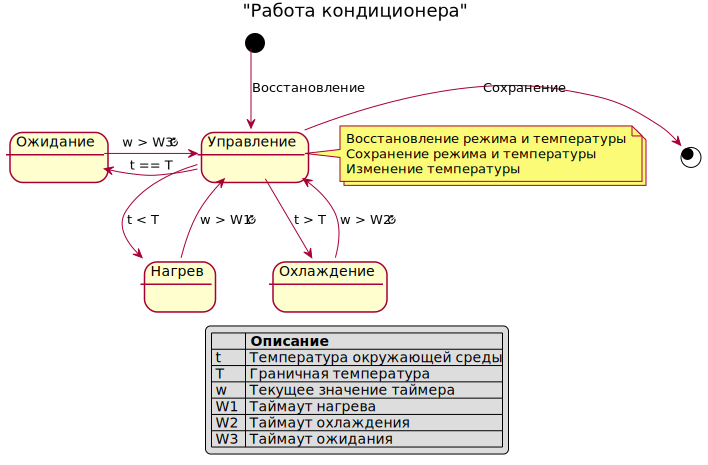
\includegraphics[width=\textwidth]{cond_sample}
  \centering
    \caption{Диаграмам состояний работы кондиционера}
  \label{fig:cond_diagram}
\end{figure}

Давайте более детально рассмотрим текст описания диаграммы.
Ключевое слово \texttt{@startuml} начинает блок описания диаграмы, а \texttt{@enduml} завершает его. \texttt{title} задает наименование нашей диаграмы. 
\texttt{legend} начинает блок легенды диаграмы, а \texttt{end legend} завершает ее. Внутри легенды пиведена конструкция задания таблицы, в которой мы описываем 
необходимые нам параметры. Состояния начала и окончания задаются при помощи \texttt{[*]} последовательности. Стрелочки \texttt{-->} задают переходы 
между состояниями, а \texttt{:} задают условия переходов. \texttt{note right of} добавляет подсказку к состоянию.

Подробности использования языка \texttt{PlantUML} можно найти по ссылке \url{http://plantuml.com/PlantUML_Language_Reference_Guide.pdf}

\newpage
\section*{Модель \texttt{Promela}}\label{practical_work_2}
\addcontentsline{toc}{section}{Модель \texttt{Promela}}
\lhead{Модель \texttt{Promela}}

\newpage
\chapter*{Лабораторные работы}\label{labs_works}
\addcontentsline{toc}{chapter}{Лабораторные работы}
\lhead{Лабораторные работы}

\section*{Задания}\label{lab_work_formatting}
\addcontentsline{toc}{section}{Задания}
\lhead{Задания}

\begin{enumerate}
  \item Светофор с индикацией оставшегося времени
  \item Грузовой лифт
  \item Автомобильный манипулятор
  \item Супервизор(управление процессами)
  \item Автоматический нагреватель воды
  \item Дренажный насос
  \item Холодильник
  \item Турникет метро
  \item Банковский терминал выдачи наличных
  \item Парковка
  \item СКУД
  \item ЧПУ фрезер
\end{enumerate}

Номер работы вычисляется путем взятия номера по порядку вышей записи в журнале старосты по модулю 12 
и прибавлением к получившемуся числу 1 ($(N mod 12) + 1$).

\section*{Требования к оформлению кода}\label{lab_work_formatting}
\addcontentsline{toc}{section}{Требования к оформлению кода}
\lhead{Требования к оформлению кода}


\section*{Требования к оформлению работы}\label{lab_work_}
\addcontentsline{toc}{section}{Требования к оформлению работы}
\lhead{Требования к оформлению работы}

Лабораторная работа должна состоять из следующих необходимых компонент:
\begin{itemize}
  \item[ 1 лист ] Титульный лист
  \item[ 2 лист ] Описание объекта управления(цели и задачи объекта управления, функциональные требования). Пример \nameref{practical_work_1}.
  \item[ 3 лист ] Модель \texttt{Promela}. Пример \nameref{practical_work_2}.
  \item[ 4 лист ] Диаграмма переходов. Пример \nameref{practical_work_1}.
  \item[ 5 лист ] Описание модулей
\end{itemize}

Работа считается принятой если выполнены условия:
\begin{enumerate}
  \item Лабораторная работа представлена в бумажном виде и состоит, как минимум, из описанных выше компонент
  \item На электронном носителе или в репозитории(\texttt{GitHub}) присутствуют в электронном виде:
    \begin{enumerate}
      \item Исходный код работы выполненный при помощи языка Си и оформленный в соответствии с требованиями \nameref{lab_work_formatting}
      \item Текст лабораторной работы в формате \texttt{doc} или \texttt{tex}
      \item Собранный исполняемы модуль приложения
      \item Проект вашей работы(файлы сборки - \texttt{cmake}, необходимые библиотеки - \texttt{googletest} как минимум, и т.д.)
    \end{enumerate}
  \item Ваша работа собирается на тестовом стенде, проходит верификацию модели, проходят все тесты(исполняется тестовый пример)
\end{enumerate}

\newpage
\section*{Лабораторная работа №1}\label{lab_work_1}
\addcontentsline{toc}{section}{Лабораторная работа №1}
\lhead{Лабораторная работа №1}


\newpage
\section*{Лабораторная работа №2}\label{lab_work_2}
\addcontentsline{toc}{section}{Лабораторная работа №2}
\lhead{Лабораторная работа №2}


\newpage
\chapter*{Приложение}\label{addons}
\addcontentsline{toc}{chapter}{Приложение}
\lhead{Приложение}

\section*{Описание опций \texttt{SPIN}}\label{spin_quick_REFERENCE}
\addcontentsline{toc}{section}{Описание опций \texttt{SPIN}}

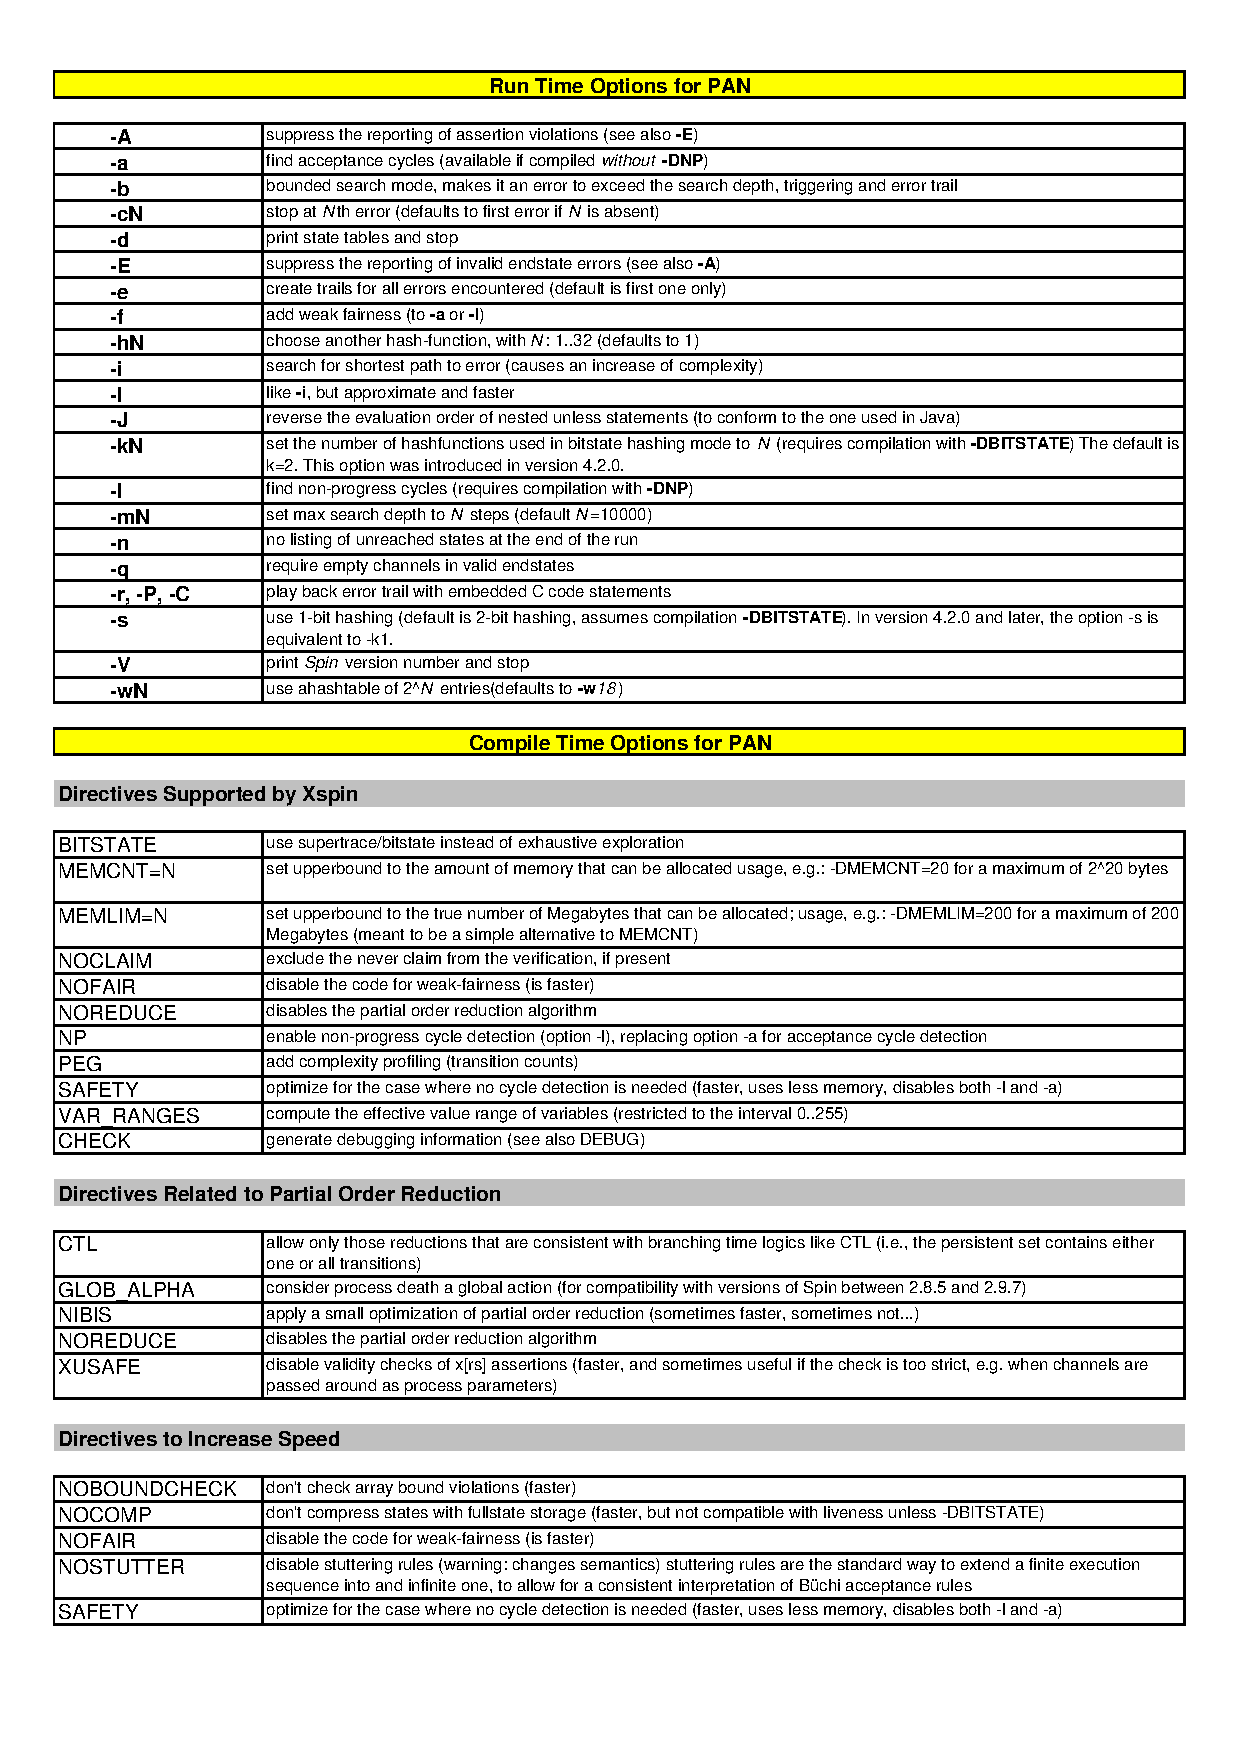
\includepdf[pages=-]{spin-quick-reference.pdf}

\section*{\texttt{BNF} Языка \texttt{Promela}}\label{promela_BNF}
\addcontentsline{toc}{section}{\texttt{BNF} Языка \texttt{Promela}}
\begin{verbatim}
spec	: module [ module ] *

module	: proctype	/* proctype declaration */
	| init		/* init process       */
	| never		/* never claim        */
	| trace		/* event trace        */
	| utype		/* user defined types */
	| mtype		/* mtype declaration  */
	| decl_lst	/* global vars, chans */

proctype: [ active ] PROCTYPE name '(' [ decl_lst ]')'
	  [ priority ] [ enabler ] '{' sequence '}'

init	: INIT [ priority ] '{' sequence '}'

never	: NEVER	'{' sequence '}'

trace	: TRACE '{' sequence '}'

utype	: TYPEDEF name '{' decl_lst '}'

mtype	: MTYPE [ '=' ] '{' name [ ',' name ] * '}'

decl_lst: one_decl [ ';' one_decl ] *

one_decl: [ visible ] typename  ivar [',' ivar ] *

typename: BIT | BOOL | BYTE | SHORT | INT | MTYPE | CHAN
	| uname	/* user defined type names (see utype) */

active  : ACTIVE [ '[' const ']' ]	/* instantiation */

priority: PRIORITY const	/* simulation priority */

enabler : PROVIDED '(' expr ')'	/* execution constraint */

visible	: HIDDEN | SHOW

sequence: step [ ';' step ] *

step    : stmnt	[ UNLESS stmnt ]
	| decl_lst
	| XR varref [',' varref ] *
	| XS varref [',' varref ] *

ivar    : name [ '[' const ']' ] [ '=' any_expr | '=' ch_init ]

ch_init : '[' const ']' OF '{' typename [ ',' typename ] * '}'

varref	: name [ '[' any_expr ']' ] [ '.' varref ]

send    : varref '!' send_args		/* normal fifo send */
	| varref '!' '!' send_args	/* sorted send */

receive : varref '?' recv_args		/* normal receive */
	| varref '?' '?' recv_args	/* random receive */
	| varref '?' '<' recv_args '>'	/* poll with side-effect */
	| varref '?' '?' '<' recv_args '>'	/* ditto */

poll    : varref '?' '[' recv_args ']'	/* poll without side-effect */
	| varref '?' '?' '[' recv_args ']'	/* ditto */

send_args: arg_lst | any_expr '(' arg_lst ')'

arg_lst  : any_expr [ ',' any_expr ] *

recv_args: recv_arg [ ',' recv_arg ] *  |  recv_arg '(' recv_args ')'

recv_arg : varref | EVAL '(' varref ')' | [ '-' ] const

assign  : varref '=' any_expr	/* standard assignment */
	| varref '+' '+'	/* increment */
	| varref '-' '-'	/* decrement */

stmnt	: IF options FI		/* selection */
	| DO options OD		/* iteration */
	| FOR '(' range ')' '{' sequence '}'		/* iteration */
	| ATOMIC '{' sequence '}'	/* atomic sequence */
	| D_STEP '{' sequence '}'	/* deterministic atomic */
	| SELECT '(' range ')'	/* non-deterministic value selection */
	| '{' sequence '}'	/* normal sequence */
	| send
	| receive
	| assign
	| ELSE			/* used inside options */
	| BREAK			/* used inside iterations */
	| GOTO name
	| name ':' stmnt	/* labeled statement */
	| PRINT '(' string [ ',' arg_lst ] ')'
	| ASSERT expr
	| expr			/* condition */
	| c_code '{' ... '}'	/* embedded C code */
	| c_expr '{' ... '}'
	| c_decl '{' ... '}'
	| c_track '{' ... '}'
	| c_state '{' ... '}'

range	: varref ':' expr '..' expr
	| varref IN varref

options : ':' ':' sequence [ ':' ':' sequence ] *

andor	: '&' '&' | '|' '|'

binarop	: '+' | '-' | '*' | '/' | '%' | '&' | '^' | '|'
	| '>' | '<' | '>' '=' | '<' '=' | '=' '=' | '!' '='
	| '<' '<' | '>' '>' | andor

unarop	: '~' | '-' | '!'

any_expr: '(' any_expr ')'
	| any_expr binarop any_expr
	| unarop any_expr
	| '(' any_expr '-' '>' any_expr ':' any_expr ')'
	| LEN '(' varref ')'	/* nr of messages in chan */
	| poll
	| varref
	| const
	| TIMEOUT
	| NP_			/* non-progress system state */
	| ENABLED '(' any_expr ')'		/* refers to a pid */
	| PC_VALUE '(' any_expr ')'		/* refers to a pid */
	| name '[' any_expr ']' '@' name	/* refers to a pid */
	| RUN name '(' [ arg_lst ] ')' [ priority ]
	| get_priority( expr )			/* expr refers to a pid */
	| set_priority( expr , expr )		/* first expr refers to a pid */

expr	: any_expr
	| '(' expr ')'
	| expr andor expr
	| chanpoll '(' varref ')'	/* may not be negated */

chanpoll: FULL | EMPTY | NFULL | NEMPTY

string	: '"' [ any_ascii_char ] * '"'

uname	: name

name	: alpha [ alpha | number ] *

const	: TRUE | FALSE | SKIP | number [ number ] *

alpha	: 'a' | 'b' | 'c' | 'd' | 'e' | 'f' | 'g' | 'h' | 'i' | 'j'
	| 'k' | 'l' | 'm' | 'n' | 'o' | 'p' | 'q' | 'r' | 's' | 't'
	| 'u' | 'v' | 'w' | 'x' | 'y' | 'z'
	| 'A' | 'B' | 'C' | 'D' | 'E' | 'F' | 'G' | 'H' | 'I' | 'J'
	| 'K' | 'L' | 'M' | 'N' | 'O' | 'P' | 'Q' | 'R' | 'S' | 'T'
	| 'U' | 'V' | 'W' | 'X' | 'Y' | 'Z'
	| '_'

number	: '0' | '1' | '2' | '3' | '4' | '5' | '6' | '7' | '8' | '9'
\end{verbatim}

\newpage
\section*{Примеры исходного кода}
\addcontentsline{toc}{section}{Примеры исходного кода}
\lstset{
  numbers = left,
  stepnumber = 1,
  numberstyle = \fontsize{11.5pt}{0.75em}\selectfont\monaco\color{comment},
}

\begin{lstlisting}[label={monitors_cxx_account_example}, caption={Пример \texttt{C}}]
printf("Hello")
\end{lstlisting}

%-----------------------------------------%
\newpage
\thispagestyle{empty}
\bibliographystyle{abbrv}
\bibliography{bibs}
%-----------------------------------------%
\newpage
\listoffigures
\end{document}
